\chapter{Python}
\begin{center}
  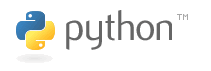
\includegraphics[width=140px]{img/python.png} \\
  \textbf{\url{http://python.org}}
\end{center}
\begin{quote}
  \textit{Python is a programming language that lets you work more quickly and integrate your systems more effectively.
          You can learn to use Python and see almost immediate gains in productivity and lower maintenance costs.}
\end{quote}

\section{IPython}
Python selbst kommt mit einer interaktiven Kommandozeile (genauer: einer REPL\footnote{read–eval–print loop}-Umgebung).
Um einen Einblick in die Sprache zu erhalten, ist diese eigentlich vollkommen ausreichend.
Sie bietet die Möglichkeit, interaktiv mit der Sprache in Kontakt zu kommen.
IPython erlaubt zusätzlich, auf die Shell zuzugreifen und interaktive Sitzungen zu speichern.
Gestartet wird IPython auf der Kommandozeile mit
\begin{verbatim}
ipython3
\end{verbatim}
und meldet sich (zum Beispiel hier unter OS X mit Python 3.2.3) mit der Ausgabe
\begin{verbatim}
Python 3.2.3 (default, Apr 13 2012, 00:15:25) 
Type "copyright", "credits" or "license" for more information.

IPython 0.13 -- An enhanced Interactive Python.
?         -> Introduction and overview of IPython's features.
%quickref -> Quick reference.
help      -> Python's own help system.
object?   -> Details about 'object', use 'object??' for extra details.

In [1]: 
\end{verbatim}
Um IPython zu beenden gibt es die Befehle \texttt{exit}, \texttt{exit()}, \texttt{quit}, \texttt{quit()} und natürlich \texttt{Ctrl-D}.

\section{Syntax}
Grundsätzlich ist die Python-Syntax sehr einfach und intuitiv.
In vielen Punkten erinnert sie eher an eine Scriptsprache.

\paragraph{Blöcke}
Durch Einrückung!
4 Leerzeichen (/1 Tab)

\paragraph{Semikolons}
Gibt es prinzipiell
Sind am Zeilenende aber nicht notwendig

\paragraph{???}
In einer interaktiven Sitzung (z.B. IPython) können zum Einstieg einfache mathematische Berechnungen durchgeführt werden:
\begin{verbatim}
In [1]: 1 + 2
Out[1]: 3

In [2]: 1 * 2
Out[2]: 2
\end{verbatim}

\subsection{Variablen}
Natürlich gibt es Variablen.
Dynamische Typisierung
Keine explizite Deklaration 
Ihre Verwendung ist denkbar einfach:
\begin{verbatim}
In [3]: a = 2

In [4]: a
Out[4]: 2

In [5]: b = 1 + 1

In [6]: b
Out[6]: 2
\end{verbatim}
Variablennamen können Buchstaben, Zahlen und Unterstrichte enthalten, dürfen jedoch nicht mit einer Ziffer beginnen.

\subsection{Datenstrukturen/-typen}
\begin{itemize}
  \item bool (\texttt{True}, \texttt{False})
  \item int, float, long, complex
  \item string (\texttt{'foo'}, \texttt{"bar"})
  \item Iteratoren, Generatoren, Sequenzen, …
\end{itemize}
\paragraph{Praktische Typen}
\begin{itemize}
  \item[\texttt{()}] Tupel
  \item[\texttt{[]}] Liste
  \item[\texttt{\{\}}] Dictionary 
\end{itemize}
\paragraph{Zum Beispiel}
\begin{minted}{python}
In [9]: cities = ['Dortmund', 'Hamburg', 'Berlin']

In [10]: cities[0]
Out[10]: 'Dortmund'
\end{minted}
\paragraph{Mehr Beispiele}
\begin{minted}{python}
In [1]: teams = {
   ...:         'BVB': "BV Borussia Dortmund 09",
   ...:         'S04': "FC Schalke 04",
   ...:         'FCB': "FC Bayern München"
   ...: }

In [2]: teams['BVB']
Out[2]: 'BV Borussia Dortmund 09'
\end{minted}


\subsection{Operatoren}
Wie aus dem obigen Beispiel hervorgeht, gibt es in Python \textbf{mathematische Operatoren}.
In \autoref{tab:op_mat} sind diese dargestellt.

\begin{table}[H]
  \centering{}
  \caption{Mathematische Operatoren}
  \label{tab:op_mat}
  \begin{tabular}{c l c c}
    \toprule
    Op.         & Funktion         & Beispiel         & Ergebnis \\
    \midrule
    \texttt{+}  & Addition         & \texttt{1 + 2}   & \texttt{3} \\
    \texttt{-}  & Subtraktion      & \texttt{1 - 2}   & \texttt{-1} \\
    \texttt{*}  & Multiplikation   & \texttt{1 * 2}   & \texttt{2} \\
    \texttt{/}  & Division         & \texttt{1 / 2}   & \texttt{0.5} \\
    \texttt{\%} & Modulo           & \texttt{11 \% 2} & \texttt{1} \\
    \texttt{**} & Exponent         & \texttt{2**3}  & \texttt{8} \\
    \texttt{//} & Ganzzahldivision & \texttt{5 // 2}  & \texttt{2} \\
    \bottomrule
  \end{tabular}
\end{table}

\textbf{Zuweisungsoperatoren} setzen sich aus einem mathematischen Operator und einem Gleichheitszeichen zusammen.
Mit ihnen kann gleichzeitig eine Berechnung und eine Zuweisung durchgeführt werden, zum Beispiel:
\begin{verbatim}
In [7]: a = 2

In [7]: a *= 3

In [8]: a
Out[8]: 6
\end{verbatim}

Mit Hilfe von \textbf{Vergleichsoperatoren} (siehe \autoref{tab:op_comp}) lassen sich Vergleiche durchführen.
\begin{table}[H]
  \centering{}
  \caption{Vergleichsoperatoren}
  \label{tab:op_comp}
  \begin{tabular}{c l c c}
    \toprule
    Op.             & Funktion            & Beispiel        & Ergebnis \\
    \midrule
    \texttt{==}     & Gleich              & \texttt{1 == 1} & \texttt{True} \\
    \texttt{!=}     & Ungleich            & \texttt{2 != 1} & \texttt{True} \\
    \texttt{>}      & Größer              & \texttt{2 > 1}  & \texttt{True} \\
    \texttt{<}      & Kleiner             & \texttt{1 < 2}  & \texttt{True} \\
    \texttt{>=}     & Größer oder gleich  & \texttt{2 >= 1} & \texttt{True} \\
    \texttt{<=}     & Kleiner oder gleich & \texttt{1 <= 2} & \texttt{True} \\
    \bottomrule
  \end{tabular}
\end{table}

\paragraph{Logische Operatoren}
\begin{minted}{python}
and, or, not
\end{minted}
\paragraph{Identitätsoperatoren}
\begin{minted}{python}
is, is not
\end{minted}
\paragraph{Operatoren für Sequenzen}
\begin{minted}{python}
in, not in
\end{minted}


\subsection{Dateien} 
python
    open
    file
        write
    range
    len
    string
        format
        join
    list
        append
        index
    dict
    sorted
    decimal
    math
        floor
        ceil
    convert
        str
        int
        float

\subsection{Bibliotheken}
\subsubsection{PyLab}
\begin{frame}{PyLab}
  \begin{itemize}
    \item bündelt NumPy, SciPy und Matplotlib
    \item starten mit \texttt{ipython3 --pylab}
  \end{itemize}
\end{frame}

\subsubsection{NumPy}
\begin{frame}{NumPy}
  \begin{center}
    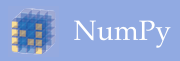
\includegraphics[width=100px]{../Notes/img/numpy.png}
  \end{center}
  \begin{itemize}
    \item $n$-dimensionale Arrays
    \item Funktionen, die auf denen arbeiten
    \item Operatoren wirken elementweise
    \item wird meist mit \texttt{np} abgekürzt
  \end{itemize}

  Konstanten:
  \begin{itemize}
    \item \texttt{pi}
    \item \texttt{e}
  \end{itemize}
\end{frame}

\begin{frame}{Arrays erstellen}
  \begin{itemize}
    \item \texttt{array}: konvertiert irgendwas (Liste, Tupel, …) zu einem Array
    \item \texttt{linspace(start, end, number)}: Array aus \texttt{number} Zahlen zwischen \texttt{start} und \texttt{end} in gleichem Abstand
    \item \texttt{arange(start, end, step)}: Array aus Zahlen zwischen \texttt{start} und \texttt{end} mit dem Abstand \texttt{step}
    \item \texttt{zeros(shape)}: Array aus Nullen der Größe \texttt{shape}
    \item \texttt{ones(shape)}: Array aus Einsen der Größe \texttt{shape}
  \end{itemize}
\end{frame}

\begin{frame}{Elementweise Funktionen}
  Beispiele:
  \begin{itemize}
    \item \texttt{sqrt}
    \item \texttt{exp}, \texttt{log}
    \item \texttt{sin}
    \item \texttt{deg2rad}, \texttt{rad2deg}
  \end{itemize}
\end{frame}

\begin{frame}{Reduzierende Funktionen}
  Beispiele:
  \begin{itemize}
    \item \texttt{sum}
    \item \texttt{mean}
    \item \texttt{max}, \texttt{min}
    \item \texttt{ediff1d}
  \end{itemize}
\end{frame}

\begin{frame}{It/Output}
  \begin{itemize}
    \item \texttt{loadtxt(file [, unpack=True])}: Lädt eine Datei in ein Array.
      \texttt{unpack=True} transponiert das Array
    \item \texttt{savetxt(file, array)}: Speichert ein Array in eine Datei
  \end{itemize}
\end{frame}

\subsubsection{SciPy}
\begin{frame}{SciPy}
  \begin{center}
    
\includegraphics{../Notes/img/scipy.pdf}
  \end{center}
\end{frame}

\begin{frame}{Nützliche Funktionen}
  \begin{itemize}
    \item \texttt{optimize.curve\_fit}: fittet nichtlineare Funktionen
    \item \texttt{stats.sem}: gibt den Fehler des Mittelwerts
    \item \texttt{constants.C2K}: konvertiert Celsius in Kelvin
    \item \texttt{constants.K2C}: konvertiert Kelvin in Celsius
  \end{itemize}
\end{frame}

\begin{frame}{Konstanten}
  \begin{itemize}
    \item \texttt{constants.physical\_constants}: enthält diverse physikalische Konstanten, ihre Fehler und Einheiten (aus CODATA)
  \end{itemize}
\end{frame}

\subsubsection{matplotlib}
\begin{frame}{matplotlib}
  \begin{center}
    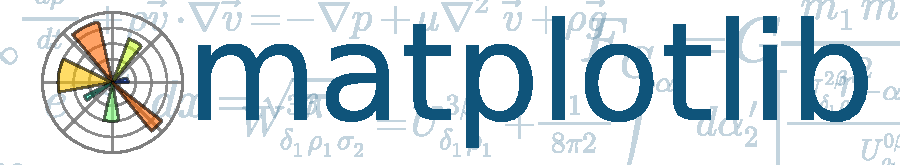
\includegraphics[width=\textwidth]{../Notes/img/matplotlib.pdf}
  \end{center}
  \begin{itemize}
    \item prozedurales Interface (pyplot, in PyLab) \mdash\ einfacher
    \item objektorientiertes Interface (Beschreibung im Skript) \mdash\ flexibler, schöner für größere Skripte oder Programme
  \end{itemize}
\end{frame}

\begin{frame}{Beispiele}
  \begin{center}
    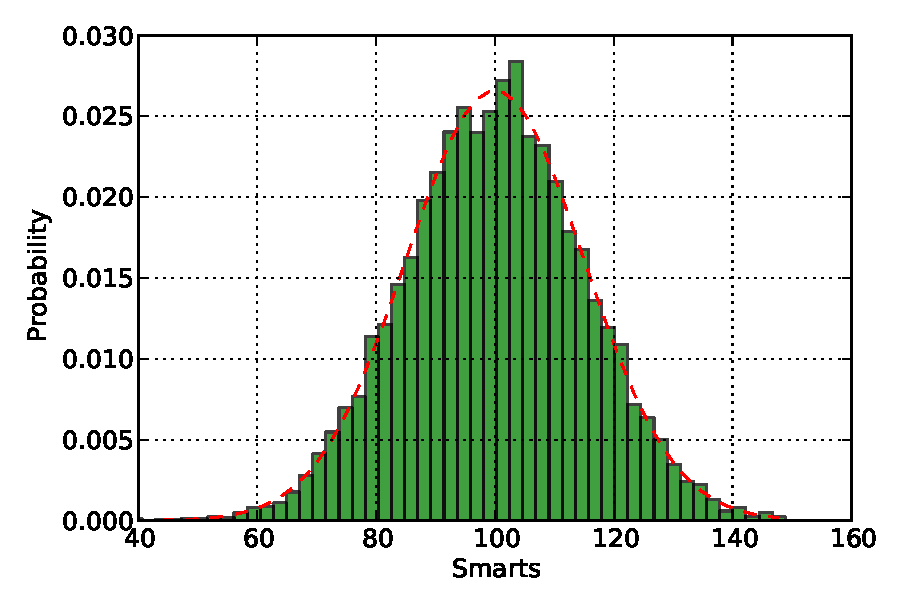
\includegraphics[width=0.8\textwidth]{img/matplotlib/hist.pdf}
  \end{center}
\end{frame}

\begin{frame}{Beispiele}
  \begin{center}
    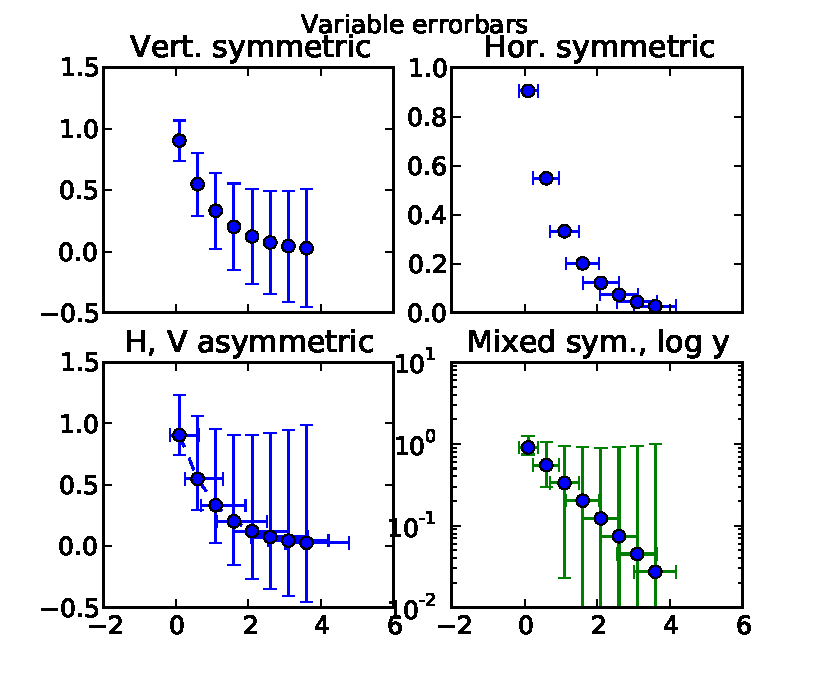
\includegraphics[width=0.8\textwidth]{img/matplotlib/errorbars.pdf}
  \end{center}
\end{frame}

\begin{frame}{Beispiele}
  \begin{center}
    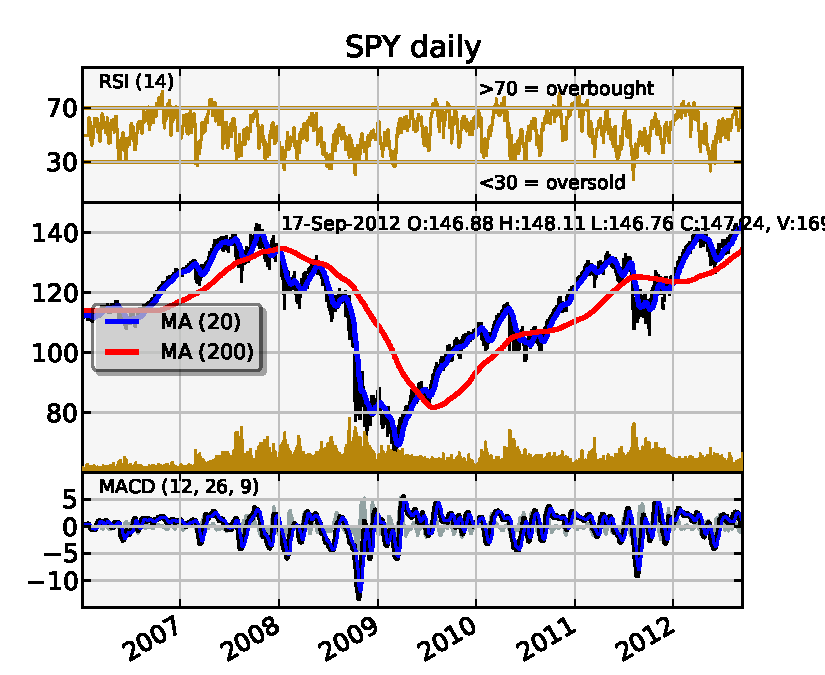
\includegraphics[width=0.8\textwidth]{img/matplotlib/finance.pdf}
  \end{center}
\end{frame}

\begin{frame}{Beispiele}
  \begin{center}
    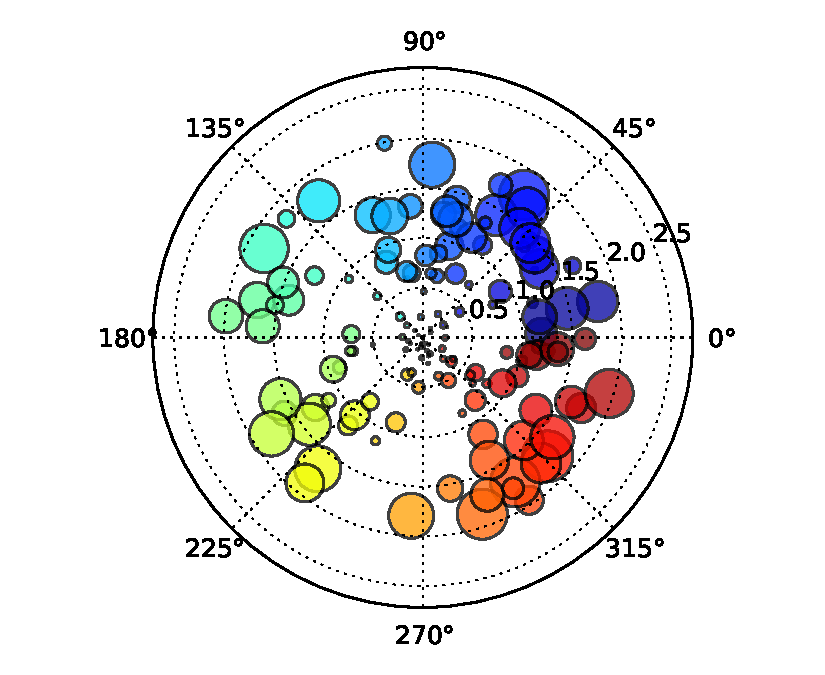
\includegraphics[width=0.8\textwidth]{img/matplotlib/polar.pdf}
  \end{center}
\end{frame}

\begin{frame}{Beispiele}
  \begin{center}
    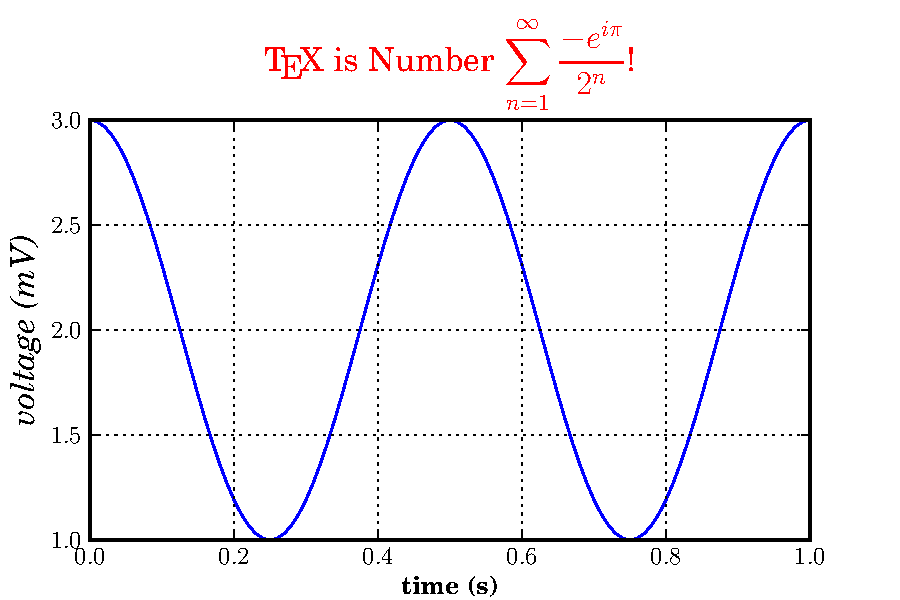
\includegraphics[width=0.8\textwidth]{img/matplotlib/tex.pdf}
  \end{center}
\end{frame}

\begin{frame}{Beispiele}
  \begin{center}
    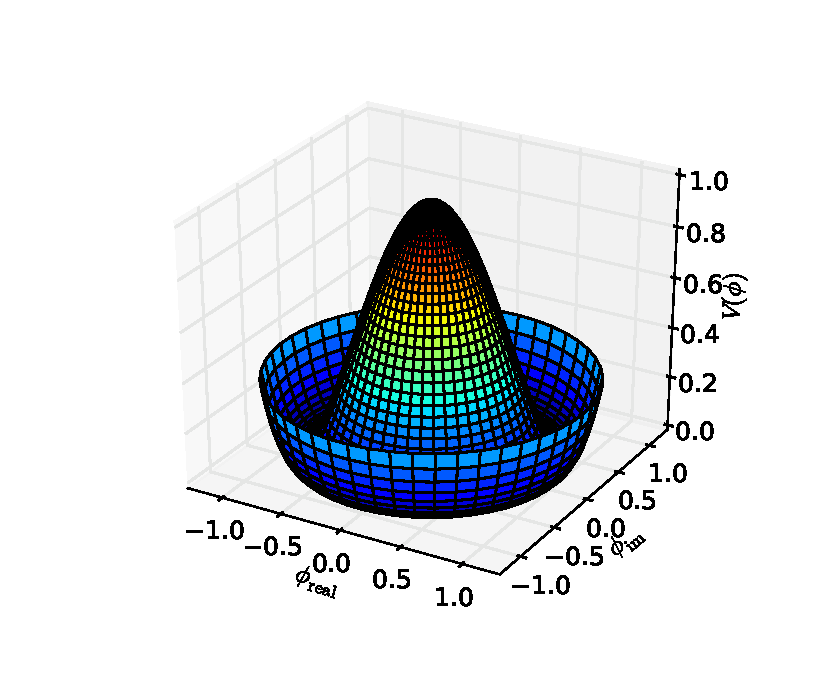
\includegraphics[width=0.8\textwidth]{img/matplotlib/mplot3d.pdf}
  \end{center}
\end{frame}

\begin{frame}[fragile]{Plotten mit IPython}
  Einfach \texttt{ipython3 --pylab} ausführen und z.B. Folgendes eintippen:
\begin{minted}{python}
  In [1]: x = linspace(0, 1, 100)
  In [2]: plot(x, x**2, 'b-')
\end{minted}
  An dem Plot kann interaktiv weiter gearbeitet werden.
\end{frame}

\begin{frame}[fragile]{Plots in .py-Dateien erstellen}
  In Code-Dateien muss man erst einmal die passenden Bibliotheken importieren.\\
  Außerdem erscheint der Plot erst, wenn man \verb|show()| aufruft.
\begin{minted}{python}
from numpy import linspace, pi, sin
import matplotlib.pyplot as plt
x = linspace(0, 2 * pi, 1000)
plt.plot(x, sin(x), 'r--')
plt.show()
# oder: plt.savefig('plot.pdf')
\end{minted}
\end{frame}

\begin{frame}{Verschiedene Arten von Plots}
  \begin{itemize}
    \item \texttt{plot}
    \item \texttt{errorbar} - Plot mit Fehlerbalken
    \item \texttt{semilogy}, \texttt{semilogx} - logarithmische Skalierung
    \item \texttt{hist} - Histogramme
    \item Polare Plots funktionieren mit dem objektorientierten Interface.
  \end{itemize}
\end{frame}

\begin{frame}{Nützliche Funktionen}
  \begin{itemize}
    \item \texttt{title('...')}
    \item \texttt{xlabel('...'), ylabel('...')}
    \item \texttt{clf()}
  \end{itemize}
\end{frame}



\section{Python 2}
Falls man Python 2 verwendet, sollte jede \texttt{.py}-Datei so anfangen:
\begin{verbatim}
# coding=utf-8
from __future__ import division, print_function, unicode_literals
\end{verbatim}
Dann funktionieren Division, \texttt{print} und Unicode wie in Python 3.
Man sollte dann auch immer \texttt{python2} und \texttt{ipython2} aufrufen.

\section{Weiterführende Links}
\begin{itemize}
  \item Learn Python The Hard Way (Python 2): \url{http://learnpythonthehardway.org/}
  \item Dive Into Python 3: \url{http://www.diveintopython3.net/}
  \item Python v3 documentation: \url{http://docs.python.org/py3k/}
  \item PEP 8 -- Style Guide for Python Code: \url{http://www.python.org/dev/peps/pep-0008/}
  \item Tentative NumPy Tutorial: \url{http://www.scipy.org/Tentative\_NumPy\_Tutorial}
  \item NumPy and SciPy Documentation: \url{http://docs.scipy.org/doc/}
  \item matplotlib Documentation: \url{http://matplotlib.org/1.2.0/contents.html}
  \item matplotlib Gallery: \url{http://matplotlib.org/1.2.0/gallery.html}
  \item Python Uncertainties package: \url{http://packages.python.org/uncertainties/}
  \item SymPy: \url{http://sympy.org/en/index.html}
  \item matplotlib tutorial: \url{http://www.loria.fr/~rougier/teaching/matplotlib/}
  \item Python Scientific Lecture Notes: \url{http://scipy-lectures.github.com/}
  \item PyCon 2012: \url{http://pyvideo.org/category/17/pycon-us-2012}
    \begin{itemize}
      \item Plotting with matplotlib: \url{http://pyvideo.org/video/617/plotting-with-matplotlib}
      \item IPython: Python at your fingertips: \url{http://pyvideo.org/video/640/ipython-python-at-your-fingertips}
      \item IPython in-depth: high-productivity interactive and parallel python: \url{http://pyvideo.org/video/605/ipython-in-depth-high-productivity-interactive-a}
      \item Python for data lovers: explore it, analyze it, map it: \url{http://pyvideo.org/video/676/python-for-data-lovers-explore-it-analyze-it-m}
      \item Sage: Open Source Math in Python: \url{http://pyvideo.org/video/652/sage-open-source-math-in-python}
    \end{itemize}
  \item SciPy 2012: \url{http://pyvideo.org/category/20/scipy\_2012}
    \begin{itemize}
      \item Introduction to NumPy and matplotlib: \url{http://pyvideo.org/video/1190/introduction-to-numpy-and-matplotlib}
      \item Advanced matplotlib: \url{http://pyvideo.org/video/1344/advanced-matplotlib}
      \item IPython: tools for the entire lifecycle of research computing: \url{http://pyvideo.org/video/1221/ipython-tools-for-the-entire-lifecycle-of-resear}
      \item A tale of four libraries: \url{http://pyvideo.org/video/1211/a-tale-of-four-libraries}
    \end{itemize}
  \item SciPy 2011: \url{http://archive.org/search.php?query=subject\%3A\%22SciPy2011\%22}
\end{itemize}
